\chapter{Neural Networks Compression}
-Model compression encompasses a family of techniques aimed at reducing the computational and memory demands of neural networks while preserving, as much as possible, their predictive performance. These methods are typically applied at the level of layers, submodules, or parameter groups and introduce explicit trade-offs between efficiency metrics and model accuracy. Key objectives include reducing model size, lowering inference latency, decreasing memory bandwidth usage, and accelerating both training and deployment, particularly in resource-constrained environments.

A notable characteristic of modern deep learning models is their heavy overparameterization. In such regimes, compression does not merely remove redundancy but can also act as an implicit form of regularization, mitigating overfitting and occasionally improving generalization performance. This phenomenon has been observed across a variety of architectures, especially in large-scale transformer-based models.

Among the most widely adopted compression strategies are \emph{pruning}, \emph{quantization}, \emph{knowledge distillation}, and \emph{low-rank factorization}. Pruning methods remove parameters, neurons, attention heads, or entire structural components deemed redundant or unimportant according to some saliency criterion, thereby inducing sparsity in the network. Quantization reduces numerical precision by representing weights, activations, or gradients with fewer bits, leading to significant gains in memory efficiency and hardware throughput. Knowledge distillation transfers information from a high-capacity teacher model to a smaller student model by matching output distributions or intermediate representations, enabling compact models to retain much of the teacher’s behavior. Low-rank factorization exploits linear dependencies in weight matrices by decomposing them into products of smaller matrices, effectively reducing parameter count and computational complexity without altering the overall network topology.

These techniques are not mutually exclusive and are frequently combined in practice. Hybrid compression pipelines leverage their complementary strengths to achieve higher compression ratios and better efficiency–accuracy trade-offs than any single method alone.

\section{Quantization}


Quantization is the approximation of continuous-valued signals with a finite set of discrete values that can be represented either as integers or reduced-precision floating-point numbers. The method has a long history in information theory and signal processing \cite{gray1998quantization} as it forms the basis of analog-to-digital conversion (ADC) and helps with compact digital representations of physical measurements \cite{pelgrom2010adc}, we can also see that the same principle does appear in computational and machine learning systems, for example, early neural network models used quantized representations to induce grammatical structure and to support the learning of formal syntactic features of regular grammar for example. \cite{giles-miller-gi-1991}.

When applied to machine learning models, quantization typically replaces high precision floating-point representations of weights and activations with lower-precision types (for example, 8-bit integers or low-bit floating formats). The immediate advantages are reduced model size and reduced memory traffic; both effects directly alleviate the memory wall problem and can enable inference on cheaper or constrained hardware platforms \cite{krishnamoorthi2018,baum2023fitting}. In practice, specialized hardware and software stacks also exploit narrower data types to accelerate arithmetic, so throughput improvements are commonly observed when models are quantized and correctly supported by the execution stack \cite{krishnamoorthi2018,baum2023fitting}.

Lowering numeric precision is not free: rounding and reduced dynamic range introduce quantization error, and naive quantization can degrade model accuracy. Nevertheless, modern methods that ranges from per-channel scaling and calibration to quantization-aware training and advanced post-training schemes which often keep performance losses small; recent transformer-specific work shows that careful PTQ and FP-style low-bit representations can yield good results even at extreme 4-bit quantization. \cite{liu-etal-2023-llm}

Another practical consideration is computational overhead. Quantize/dequantize operations and the bookkeeping needed for group-wise or per-channel scales introduce extra computations relative to a pure floating-point pipeline. Yet, because quantization reduces the volume of data that must be moved between memory hierarchies and because many chips perform narrower-width operations more efficiently, end-to-end latency and energy consumption can still improve despite those extra steps \cite{krishnamoorthi2018,baum2023fitting}.

In short, the modest loss in numerical fidelity from quantization often yields large practical gains in memory footprint, throughput and power use, which is why quantization has become an indispensable tool for deploying large models in production and on-edge environments \cite{krishnamoorthi2018,liu-etal-2023-llm}.

\begin{figure}[h!]
  \centering
  \makebox[\textwidth][c]{%
    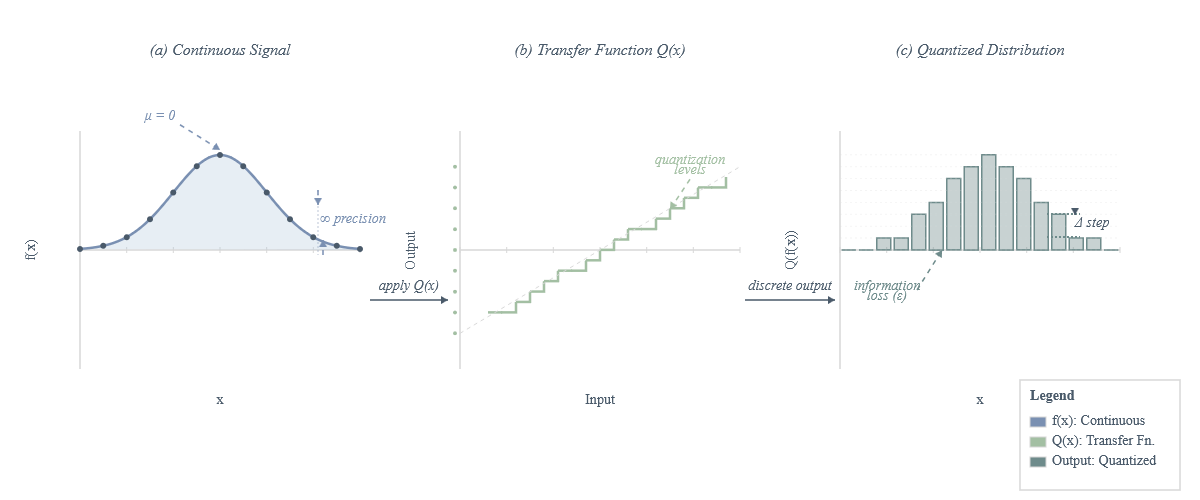
\includegraphics[scale=0.5]{quantization.png}%
  }
  \caption{Quantization of a normal distribution value $x$ into $n$ precision bits. The quantized value is computed as $Q(x) = \lfloor x \cdot 2^n \rfloor / 2^n$, and the quantization error $\varepsilon = |x - Q(x)|$}
  \label{fig:quantization_example}
\end{figure}

\subsection{Data Types used in Machine Learning}

\sunsubsection{Floating-Point Formats}

In the realm of deep learning training, the most prevalent floating-point formats are IEEE 754 Single Precision (FP32), Half Precision (FP16) \cite{micikevicius2017mixed}, and the Brain Floating Point (BFloat16 or BF16) \cite{kalamkar2019study}.

A floating-point number is structurally divided into bits allocated for the sign, the exponent, and the mantissa (significand). This structure allows for the representation of a vast range of values. Mathematically, a floating-point value $z$ is defined as:

\begin{equation}
  z = (-1)^s \times \left(1 + \frac{\hat{m}}{2^M}\right) \times 2^{\hat{e}-B}
  \label{eq:float}
\end{equation}

\noindent where $s$ represents the sign bit, $\hat{m}$ is the integer value of the mantissa comprising $M$ bits, $\hat{e}$ is the integer value of the exponent comprising $E$ bits, and $B$ is the exponent bias.

The trade-offs between these formats are visualized in Figure \ref{fig:dtypes} and summarized as follows:

\begin{itemize}
  \item \textbf{FP16:} By reducing the total bit count to 16, FP16 reduces memory bandwidth and storage requirements by $2\times$ compared to FP32. However, the reduced number of exponent bits shrinks the dynamic range, which can lead to numerical instability (e.g., underflow or overflow) during training.
  \item \textbf{BFloat16:} This format also provides a $2\times$ reduction in memory usage compared to FP32. Crucially, BFloat16 maintains the same number of exponent bits ($E=8$) as FP32, thereby preserving the full dynamic range of single-precision arithmetic \cite{kalamkar2019study}. This balance between the speed of half-precision and the range of single-precision makes BF16 a preferred standard for modern model training.
\end{itemize}

\begin{figure}[H]
  \centering
  \begin{tikzpicture}
    % Configuration
    \def\barheight{0.8}
    \def\totalwidth{12} % cm

    % FP32 Construction
    % 1 Sign, 8 Exp, 23 Mantissa = 32 total
    \node[anchor=west] at (0, 1.5) {\textbf{FP32} (32-bit)};

    % Sign
    \fill[signcol] (0,0) rectangle ++({1/32*\totalwidth}, \barheight);
    \node[white, font=\tiny] at ({0.5/32*\totalwidth}, \barheight/2) {S};

    % Exponent
    \fill[expcol] ({1/32*\totalwidth},0) rectangle ++({8/32*\totalwidth}, \barheight);
    \node[white, font=\tiny] at ({5/32*\totalwidth}, \barheight/2) {Exponent (8)};

    % Mantissa
    \fill[mantcol] ({9/32*\totalwidth},0) rectangle ++({23/32*\totalwidth}, \barheight);
    \node[white, font=\tiny] at ({20.5/32*\totalwidth}, \barheight/2) {Mantissa (23)};

    % Range vs Precision Arrow for FP32
    \draw[<->, gray] (0, -0.2) -- ({9/32*\totalwidth}, -0.2) node[midway, below, font=\tiny] {Range};
    \draw[<->, gray] ({9/32*\totalwidth}, -0.2) -- (\totalwidth, -0.2) node[midway, below, font=\tiny] {Precision};

    % BF16 Construction
    % 1 Sign, 8 Exp, 7 Mantissa = 16 total
    \begin{scope}[yshift=-2.5cm]
      \node[anchor=west] at (0, 1.5) {\textbf{BFloat16} (16-bit)};

      % Sign
      \fill[signcol] (0,0) rectangle ++({1/32*\totalwidth}, \barheight);
      \node[white, font=\tiny] at ({0.5/32*\totalwidth}, \barheight/2) {S};

      % Exponent (Same width as FP32)
      \fill[expcol] ({1/32*\totalwidth},0) rectangle ++({8/32*\totalwidth}, \barheight);
      \node[white, font=\tiny] at ({5/32*\totalwidth}, \barheight/2) {Exponent (8)};

      % Mantissa
      \fill[mantcol] ({9/32*\totalwidth},0) rectangle ++({7/32*\totalwidth}, \barheight);
      \node[white, font=\tiny] at ({12.5/32*\totalwidth}, \barheight/2) {Mant. (7)};

      % Empty space to show it is shorter
      \draw[dashed] ({16/32*\totalwidth},0) rectangle ++({16/32*\totalwidth}, \barheight);
      \node[gray, font=\tiny] at ({24/32*\totalwidth}, \barheight/2) {Saved Memory};
    \end{scope}

    % FP16 Construction
    % 1 Sign, 5 Exp, 10 Mantissa = 16 total
    \begin{scope}[yshift=-5cm]
      \node[anchor=west] at (0, 1.5) {\textbf{FP16} (16-bit)};

      % Sign
      \fill[signcol] (0,0) rectangle ++({1/32*\totalwidth}, \barheight);
      \node[white, font=\tiny] at ({0.5/32*\totalwidth}, \barheight/2) {S};

      % Exponent
      \fill[expcol] ({1/32*\totalwidth},0) rectangle ++({5/32*\totalwidth}, \barheight);
      \node[white, font=\tiny] at ({3.5/32*\totalwidth}, \barheight/2) {Exp (5)};

      % Mantissa
      \fill[mantcol] ({6/32*\totalwidth},0) rectangle ++({10/32*\totalwidth}, \barheight);
      \node[white, font=\tiny] at ({11/32*\totalwidth}, \barheight/2) {Mantissa (10)};

      % Empty space
      \draw[dashed] ({16/32*\totalwidth},0) rectangle ++({16/32*\totalwidth}, \barheight);
      \node[gray, font=\tiny] at ({24/32*\totalwidth}, \barheight/2) {Saved Memory};
    \end{scope}

  \end{tikzpicture}
  \caption{Visual comparison of bit allocation in FP32, BFloat16, and FP16 formats. Note that BFloat16 preserves the exponent width of FP32 to maintain dynamic range, while FP16 allocates more bits to the mantissa for precision at the cost of range.}
  \label{fig:dtypes}
\end{figure}

Once training concludes, models are often quantized by converting weights and activations from floating-point to integer representations, that is done to facilitate efficient deployment.

\subsubsection{Integer Formats}

Integer quantization is a critical technique for reducing model size and latency. The most widely adopted format is INT8 \cite{jacob2018quantization, dettmers2022llm}, followed by more aggressive compression formats like INT4 \cite{wu2023understanding}. Extreme quantization techniques can even reduce precision to binary formats \cite{hubara2016binarized}, yielding maximal reductions in memory footprint.

Integer formats utilize a simpler structural representation compared to floating-point numbers, enabling more efficient arithmetic logic units (ALUs). A quantized integer value is typically mapped to a real value using an affine transformation:

\begin{equation}
  z = s \times (\hat{z} - z_{zero})
  \label{eq:int}
\end{equation}

\noindent or, as often simplified in symmetric quantization schemes:

\begin{equation}
  z = s \times \hat{z} + b
\end{equation}

\noindent where $s$ is a strictly positive scale factor, $b$ is a bias term (related to the zero-point), and $\hat{z}$ represents the discrete integer value composed of $N$ bits (e.g., $N=8$ for INT8).

\begin{figure}[H]
  \centering
  \begin{tikzpicture}
    % Memory footprint comparison
    \begin{axis}[
        ybar,
        width=12cm,
        height=5cm,
        ylabel={Memory Footprint (Relative to FP32)},
        symbolic x coords={FP32, BF16, FP16, INT8, INT4, Binary},
        xtick=data,
        ymin=0, ymax=1.1,
        bar width=20pt,
        nodes near coords,
        nodes near coords align={vertical},
        title={Relative Memory Footprint by Data Type},
        legend pos=north east,
      ]
      \addplot[fill=signcol!70] coordinates {
        (FP32, 1.0)
        (BF16, 0.5)
        (FP16, 0.5)
        (INT8, 0.25)
        (INT4, 0.125)
        (Binary, 0.03125)
      };
    \end{axis}
  \end{tikzpicture}
  \caption{Relative memory footprint of different numerical formats normalized to FP32. Each reduction in bit-width yields proportional memory savings, with INT8 providing a 4× reduction and INT4 providing an 8× reduction compared to FP32.}
  \label{fig:memory_footprint}
\end{figure}

\subsection{Comparative Analysis}

Table \ref{tab:format_comparison} provides a comprehensive comparison of the key characteristics across different numerical formats used in machine learning.

\begin{table}[ht]
  \centering
  \caption{Comparison of Numerical Formats in Machine Learning}
  \label{tab:format_comparison}
  \begin{tabular}{@{}lcccccc@{}}
    \toprule
    \textbf{Format} & \textbf{Bits} & \textbf{Sign} & \textbf{Exp} & \textbf{Mant} & \textbf{Range} & \textbf{Primary Use} \\
    \midrule
    FP32   & 32 & 1 & 8  & 23 & $\pm$10$^{38}$ & Training (Legacy) \\
    BF16   & 16 & 1 & 8  & 7  & $\pm$10$^{38}$ & Training (Modern) \\
    FP16   & 16 & 1 & 5  & 10 & $\pm$10$^{5}$  & Training (Mixed) \\
    INT8   & 8  & - & -  & -  & [-128, 127]    & Inference \\
    INT4   & 4  & - & -  & -  & [-8, 7]        & Inference (Aggressive) \\
    Binary & 1  & - & -  & -  & \{-1, 1\}      & Extreme Compression \\
    \bottomrule
  \end{tabular}
\end{table}

\subsection{Hardware Considerations}

It is important to note that hardware support for these formats varies significantly across accelerator generations.
For instance, the NVIDIA V100 GPU based on the Volta architecture does not support native BFloat16 for its tensor cores, limiting mixed-precision options~\cite{datacrunch_v100_2025}.
In contrast, the NVIDIA H100 GPU (Hopper architecture) fully supports BFLOAT16 (and FP16, TF32, FP8, INT8) on its tensor cores, offering high throughput for modern AI workloads~\cite{nvidia_h100_specs_2025,nvidia_hopper_arch_in_depth_2022}.

Using a data format that the hardware does \emph{not} natively support typically forces software emulation (or fallback on “standard” CUDA cores), which can drastically degrade performance  negating the anticipated gains or even introducing computational bottlenecks~\cite{tensorrt_support_matrix_2025}.
Indeed, frameworks optimized for tensor-core use often disable certain precisions (e.g., BF16) on older GPUs.

Figure \ref{fig:hw_support} illustrates the evolution of data type support across different GPU architectures, highlighting the trend toward more diverse format support in recent generations.

\begin{figure}[ht]
  \centering
  \begin{tikzpicture}
    \begin{axis}[
        width=12cm,
        height=6cm,
        xlabel={GPU Architecture},
        ylabel={Supported Data Types},
        symbolic x coords={V100, A100, H100},
        xtick=data,
        ytick={0,1,2,3,4,5},
        yticklabels={0, FP32, +FP16, +TF32, +BF16, +INT8/4},
        grid=major,
        title={Hardware Data Type Support Evolution},
        legend pos=north west,
      ]

      % Cumulative support
      \addplot[ybar stacked, fill=signcol!70] coordinates {
        (V100, 1) (A100, 1) (H100, 1)
      };
      \addlegendentry{FP32}

      \addplot[ybar stacked, fill=mantcol!70] coordinates {
        (V100, 1) (A100, 1) (H100, 1)
      };
      \addlegendentry{FP16}

      \addplot[ybar stacked, fill=expcol!70] coordinates {
        (V100, 0) (A100, 1) (H100, 1)
      };
      \addlegendentry{TF32}

      \addplot[ybar stacked, fill=int8col!70] coordinates {
        (V100, 0) (A100, 1) (H100, 1)
      };
      \addlegendentry{BF16}

      \addplot[ybar stacked, fill=int4col!70] coordinates {
        (V100, 0) (A100, 1) (H100, 1)
      };
      \addlegendentry{INT8/4}

    \end{axis}
  \end{tikzpicture}
  \caption{Evolution of native hardware support for different data types across NVIDIA GPU architectures.}
  \label{fig:hw_support}
\end{figure}

\section{Fundamentals of Neural Network Pruning}

Neural network pruning is a model compression strategy aimed at reducing a network's complexity while preserving its performance. The term originates in horticulture, referring to the removal of excess growth of a plant or tree, and in computer science, it has long been associated with simplifying tree structures by removing redundant nodes and edges. This idea found early success in decision-tree learning, where pruning improves generalization by discarding superfluous branches~\cite{patil2010evaluation,aksoy2005rules3}. Because feed-forward neural networks can be represented as directed acyclic graphs, this intuition is directly transferable: unnecessary connections or entire units can be removed without altering the network's fundamental structure. In practice, pruning removes individual parameters or structured groups of parameters, thereby reducing the model's memory footprint and computational cost~\cite{cheng2025survey,nguyen2017nettrim}. While a fully trained, dense model may achieve peak training performance, pruning presents a trade-off: it can potentially boost generalization by removing redundant complexity, or, in the worst case, cause a noticeable drop in performance metrics such as accuracy or perplexity.

The primary objective of pruning is to introduce sparsity into the weight matrices $\mathbf{W}$ of a neural network. A matrix $\mathbf{W}$ is defined as $p$-sparse if a fraction $p$ of its elements are zero. The effectiveness of this sparsity is measured using multiple metrics beyond simple accuracy. These include the \textbf{Parameter Count ($P$)}, where $P = \sum_{i,j} \mathbb{I}[W_{i,j} \neq 0]$ directly correlates to memory footprint; \textbf{Floating Point Operations (FLOPs)}, quantified by the reduction ratio $R_{\text{FLOP}}$; \textbf{Inference Latency ($\mathcal{L}_{\text{inf}}$)}, measuring the actual time required for inference on target hardware; and \textbf{Perplexity (PPL)}, the standard language modeling metric defined as $\exp(\mathcal{L})$.

To frame this theoretically, let $f(\cdot;\Theta)$ be a neural network with parameters $\Theta$, and $L(\Theta) = \mathbb{E}_{(x,y)\sim p}[c(f(x;\Theta),y)]$ be the expected risk. Pruning aims to obtain a sparse parameter matrix $\Theta'$ that retains the predictive performance of the dense model. This is classically formulated as a constrained optimization problem:
\begin{equation}
\label{eq:pruning_constrained}
\min_{\Theta'} \;\widehat L(\Theta')
\qquad \text{s.t.}\qquad
\|\Theta'\|_{0} \le B,
\end{equation}
where the $\ell_0$ ``norm'' counts the nonzero entries and $B$ is a sparsity budget. This constraint is typically implemented via a binary mask $M \in \{0,1\}^{n\times m}$ such that $\Theta' = M \odot \Theta$, where $\odot$ denotes the Hadamard product. Consequently, pruning becomes the search for an optimal mask $M$.

However, pruning does not naturally correspond to a single objective; it requires balancing performance degradation against sparsity levels. Treating this as a multi-objective problem leads to the concept of \emph{Pareto optimality}. A candidate solution $\Theta'$ is Pareto optimal if no other valid solution improves sparsity without worsening loss, or improves loss without reducing sparsity. The set of all such solutions forms the \emph{Pareto front}, representing the optimal trade-off curve. To make this computationally tractable, the problem is often reduced via linear scalarization:
\begin{equation}
\label{eq:scalarization}
\min_{\Theta'}\;
\lambda_{\mathrm{perf}}
\big(\widehat L(\Theta') - \widehat L(\Theta)\big)
+
\lambda_{\mathrm{spar}}\|\Theta'\|_0,
\end{equation}
where varying the weights $\lambda_{\mathrm{perf}}$ and $\lambda_{\mathrm{spar}}$ allows one to trace different operating points along the Pareto frontier.

In implementation, pruning methods generally diverge into two main branches: \textbf{Unstructured} and \textbf{Structural} pruning~\cite{he2023structured,gale2019state}. Unstructured pruning involves removing individual weights $W_{i,j}$ (setting them to zero). While this approach can achieve substantially higher sparsity (often 95\%+), the resulting irregular data access patterns often prevent commodity hardware from capitalizing on the reduced FLOP count to achieve proportional speedups~\cite{frankle2018lottery,han2015deep}. Conversely, Structural pruning removes contiguous groups of parameters, such as entire neurons, filters, attention heads, or blocks~\cite{ma2023llmpruner,sun2023simple}. This regularity allows for efficient acceleration on standard GPUs or CPUs, leading to tangible improvements in inference latency, albeit typically at lower sparsity levels (40\%--70\%) compared to unstructured methods. Table~\ref{tab:pruning_comparison} summarizes these operational trade-offs.

\begin{table}[H]
\centering
\caption{Foundational Comparison of Pruning Granularity}
\label{tab:pruning_comparison}
\begin{tabular}{@{}p{2.2cm}p{2.5cm}p{2cm}p{2.5cm}p{2.5cm}@{}}
\toprule
\textbf{Pruning Type} & \textbf{Target Unit} & \textbf{Hardware Accel.} & \textbf{Sparsity Potential} & \textbf{Optimization Focus} \\ \midrule
Unstructured & Individual Weight $W_{i,j}$ & Low (Irregular) & High (95\%+) & Model Size, Memory \\
Structural (SRP) & Neuron, Head, Filter, Block & High (Regular) & Moderate (40\%-70\%) & Inference Speedup, FLOPs \\ \bottomrule
\end{tabular}
\end{table}

\begin{figure}[H]
    \centering
    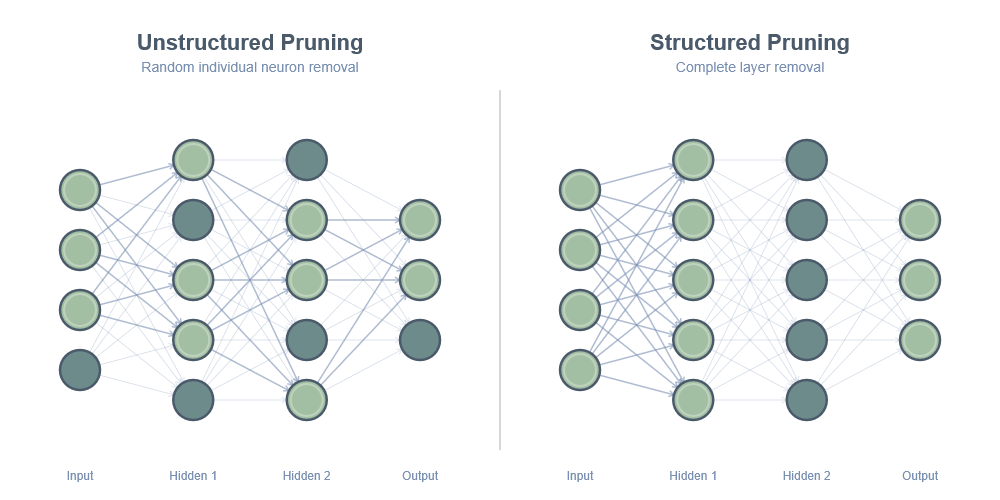
\includegraphics[scale=0.4]{canvas.png}
    \caption{The difference between unstructured pruning and structured pruning; the former removes individual neurons or weights, while the latter removes entire layers or structural blocks.}
    \label{fig:unstructured_vs_structured}
\end{figure}


\section{Low-Rank Factorization}

Low-rank factorization is a matrix decomposition technique that approximates high-dimensional matrices as products of lower-dimensional counterparts. The fundamental principle driving this approach is that deep neural network weights often exhibit significant redundancy and can be well-approximated by matrices of lower rank without a significant loss in representational capacity. This theoretical foundation was established by Li et al.~\cite{li2018measuring}, who demonstrated that the optimization landscape of deep networks is constrained to a low-dimensional manifold. In the context of large language models (LLMs), Aghajanyan et al.~\cite{aghajanyan2020intrinsic} further showed that this ``intrinsic dimensionality'' effectively predicts the success of fine-tuning regimes. When applied to architectures like the Transformer~\cite{vaswani2017attention}, low-rank factorization replaces a large weight matrix $W \in \mathbb{R}^{m \times n}$ with the product of smaller matrices $A \in \mathbb{R}^{m \times r}$ and $B \in \mathbb{R}^{r \times n}$, where $r \ll \min(m,n)$, such that:
\begin{equation}
  W \approx AB.
  \label{eq:lowrank_basic}
\end{equation}

The primary advantages of this decomposition are a reduced parameter count and a smaller memory footprint. While the original matrix requires $mn$ parameters, the factorized form requires only $r(m+n)$. As noted in the survey by Tay et al.~\cite{tay2020efficient}, this reduction is critical for deploying Transformers on memory-constrained devices, as reduced memory traffic alleviates bandwidth bottlenecks—a major performance limiter identified in works such as FlashAttention~\cite{dao2022flashattention}. The compression efficiency can be quantified by the ratio $\frac{mn}{r(m+n)}$. For instance, with dimensions $m = n = 4096$ and a rank $r = 64$, the compression ratio approaches $32\times$. However, the choice of rank $r$ introduces a fundamental trade-off between compression and model capacity. This balance is the central focus of parameter-efficient fine-tuning (PEFT) methods, most notably LoRA (Low-Rank Adaptation)~\cite{hu2021lora}, and has recently been extended to quantized models like QLoRA~\cite{dettmers2023qlora}, enabling the fine-tuning of massive parameter models on consumer hardware.

From a mathematical perspective, factorization is treated as an optimization problem minimizing the reconstruction error between the dense weight and its low-rank approximation. Formally, for a target rank $r$, we seek matrices $A$ and $B$ that minimize a distance metric, typically the Frobenius norm:
\begin{equation}
  \min_{A,B} \|W - AB\|_F^2.
  \label{eq:factorization_opt}
\end{equation}
While optimal factors correspond to the truncated Singular Value Decomposition (SVD), modern probabilistic algorithms allow for efficient computation even for massive matrices~\cite{halko2011finding}. In the specific context of Self-Attention, Wang et al.~\cite{wang2020linformer} proved in \textit{Linformer} that the attention matrix is inherently low-rank, justifying approximations that reduce complexity from $O(N^2)$ to $O(N)$. Similarly, Choromanski et al.~\cite{choromanski2020rethinking} utilized kernel-based approximations in the \textit{Performer} architecture. In modern fine-tuning scenarios, Hu et al.~\cite{hu2021lora} modified this formulation by freezing the pre-trained weights $W_0$ and learning a low-rank update $\Delta W = AB$, such that the forward pass becomes $h = W_0 x + ABx$. The success of these methods depends on rank selection; research by Ganesh et al.~\cite{ganesh2021compressing} suggests that different Transformer layers possess varying sensitivities to rank reduction, advocating for adaptive rather than uniform rank selection to minimize the normalized reconstruction error $\mathcal{E}(r) = \|W - \hat{W}_r\|_F / \|W\|_F$.

% Define colors for the TikZ figure if not already defined in preamble
\definecolor{mistyblue}{RGB}{173, 216, 230}
\definecolor{sagegreen}{RGB}{135, 175, 135}
\definecolor{dustyteal}{RGB}{95, 158, 160}
\definecolor{decompcol}{RGB}{25, 25, 112} % MidnightBlue
\definecolor{lowrankcol}{RGB}{47, 79, 79} % DarkSlateGray

\begin{figure}[h!]
  \centering
  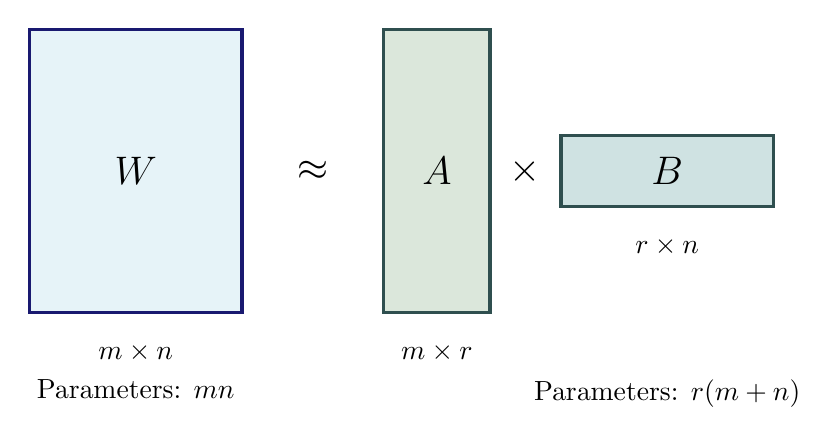
\begin{tikzpicture}[scale=0.9]
    % Original matrix
    \draw[fill=mistyblue!30, draw=decompcol, very thick] (0,0) rectangle (3,4);
    \node at (1.5,2) {\Large $W$};
    \node[below] at (1.5,-0.3) {$m \times n$};
    \node[below] at (1.5,-0.8) {Parameters: $mn$};

    % Approximately equal
    \node at (4,2) {\Large $\approx$};

    % First factor
    \draw[fill=sagegreen!30, draw=lowrankcol, very thick] (5,0) rectangle (6.5,4);
    \node at (5.75,2) {\Large $A$};
    \node[below] at (5.75,-0.3) {$m \times r$};

    % Multiplication
    \node at (7,2) {\Large $\times$};

    % Second factor
    \draw[fill=dustyteal!30, draw=lowrankcol, very thick] (7.5,1.5) rectangle (10.5,2.5);
    \node at (9,2) {\Large $B$};
    \node[below] at (9,1.2) {$r \times n$};

    % Annotation
    \node[below] at (9,-0.8) {Parameters: $r(m+n)$};
  \end{tikzpicture}
  \caption{Low-rank factorization approximates a weight matrix $W$ as a product of two smaller matrices $A$ and $B$. This structure is utilized in ALBERT \cite{lan2019albert} and LoRA \cite{hu2021lora}.}
  \label{fig:lowrank_concept}
\end{figure}


\section{Knowledge Distillation}

Knowledge Distillation (KD) is a compression paradigm effectively defined as the process of transferring "dark knowledge" from a cumbersome, high-performance model (the \textit{teacher}) to a compact, efficient model (the \textit{student}). Unlike pruning or quantization, which modify the existing weights of a model, distillation focuses on training a new, smaller architecture to mimic the behavior of a larger pre-trained one. The conceptual roots of this technique trace back to \textbf{Buciluǎ et al. \cite{bucilua2006model}}, who demonstrated model compression on ensembles, but the modern theoretical framework was solidified by \textbf{Hinton et al. \cite{hinton2015distilling}}. Their seminal work argued that the generalization capability of a large model resides not just in its final class predictions (hard labels) but in the rich, dense distribution of probabilities over all classes (soft targets). For example, in an image classification task, the probability assigned to incorrect classes reveals structural similarities; a ``BMW'' might have a low probability of being a ``garbage truck'' but a non-negligible probability of being an ``Audi.'' This side information—the relative probabilities of incorrect answers—provides a learning signal that is often more informative than the ground truth labels alone.

Mathematically, this transfer is achieved by introducing a hyperparameter $T$, known as \textit{temperature}, into the softmax function. Standard training uses $T=1$, but in distillation, the logits $z_i$ of both the teacher and student are scaled by $T$ before normalization. The probability $q_i$ for class $i$ is computed as:
\begin{equation}
    q_i = \frac{\exp(z_i / T)}{\sum_j \exp(z_j / T)}.
    \label{eq:softmax_temp}
\end{equation}
Raising $T$ produces a softer probability distribution, exposing the relationships between classes that would otherwise be suppressed by the peaking effect of the standard softmax. The training objective for the student becomes a linear combination of two loss functions: the distillation loss $L_{KD}$ (typically Kullback-Leibler divergence) which minimizes the distance between the student's and teacher's soft targets, and the standard student loss $L_{\text{task}}$ (usually Cross-Entropy) utilizing the ground truth labels. This composite objective is formulated as:
\begin{equation}
    L_{\text{total}} = \alpha T^2 L_{KD}(p_{\text{teacher}}, p_{\text{student}}) + (1-\alpha) L_{\text{task}}(y_{\text{true}}, p_{\text{student}}),
    \label{eq:kd_loss}
\end{equation}
where $\alpha$ controls the balance between mimicking the teacher and learning the hard labels. The term $T^2$ scales the gradients to ensure their magnitude remains consistent as temperature changes \cite{hinton2015distilling}.

While the original formulation focused on the final output layer (response-based knowledge), recent advancements in Transformer compression have necessitated deeper distillation strategies. \textbf{Romero et al. \cite{romero2014fitnets}} introduced \textit{FitNets}, establishing the concept of feature-based distillation, where the student learns to approximate the intermediate hidden states of the teacher. This is critical in modern architectures like BERT or GPT, where significant semantic knowledge is encoded in the internal representation layers. For instance, \textbf{DistilBERT \cite{sanh2019distilbert}} utilizes a triple loss combining language modeling, distillation, and cosine-distance loss to reduce the size of a BERT model by 40\% while retaining 97\% of its performance. More granular approaches, such as \textbf{TinyBERT \cite{jiao2020tinybert}}, extend this by distilling the attention matrices themselves, ensuring the student learns not just \textit{what} to predict, but \textit{where} to look within the input sequence. This multi-stage transfer—covering embeddings, attention maps, hidden states, and logits—ensures the student internalizes the teacher's reasoning process rather than just its final conclusions \cite{gou2021knowledge}.

\definecolor{teacherblue}{RGB}{70, 130, 180}
\definecolor{studentgreen}{RGB}{60, 179, 113}
\definecolor{lossred}{RGB}{205, 92, 92}

\begin{figure}[h!]
    \centering
    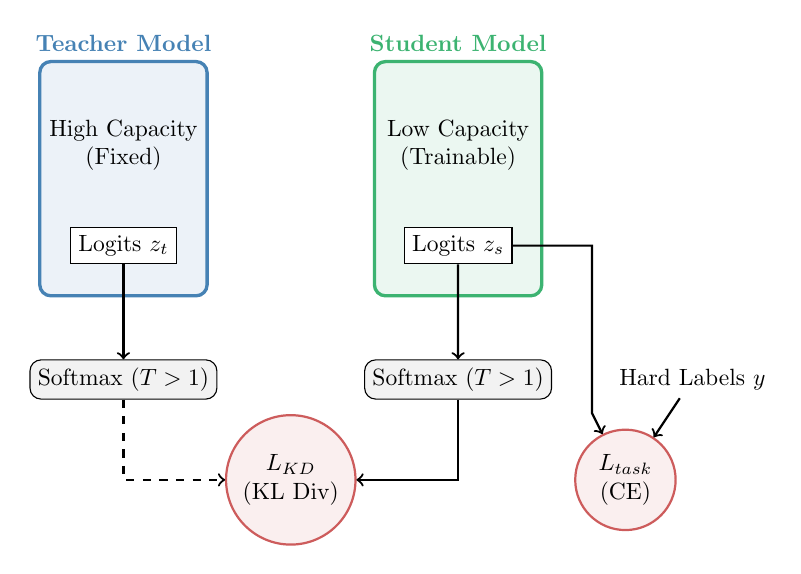
\begin{tikzpicture}[scale=0.85, every node/.style={transform shape}]
        
        % Teacher Model Block
        \node[draw=teacherblue, fill=teacherblue!10, very thick, minimum width=2.5cm, minimum height=3.5cm, rounded corners] (teacher) at (0, 2) {};
        \node[above, text=teacherblue, font=\bfseries] at (teacher.north) {Teacher Model};
        \node[align=center] at (0, 2.5) {High Capacity\\(Fixed)};
        \node[draw, fill=white] (t_logits) at (0, 1) {Logits $z_t$};
        
        % Student Model Block
        \node[draw=studentgreen, fill=studentgreen!10, very thick, minimum width=2.5cm, minimum height=3.5cm, rounded corners] (student) at (5, 2) {};
        \node[above, text=studentgreen, font=\bfseries] at (student.north) {Student Model};
        \node[align=center] at (5, 2.5) {Low Capacity\\(Trainable)};
        \node[draw, fill=white] (s_logits) at (5, 1) {Logits $z_s$};
        
        % Softmax T
        \node[draw, rounded corners, fill=gray!10] (soft_t) at (0, -1) {Softmax ($T>1$)};
        \node[draw, rounded corners, fill=gray!10] (soft_s) at (5, -1) {Softmax ($T>1$)};
        
        % Arrows
        \draw[->, thick] (t_logits) -- (soft_t);
        \draw[->, thick] (s_logits) -- (soft_s);
        
        % Distillation Loss
        \node[draw=lossred, thick, circle, minimum size=1.5cm, fill=lossred!10, align=center] (kd_loss) at (2.5, -2.5) {$L_{KD}$\\(KL Div)};
        
        \draw[->, thick, dashed] (soft_t) |- (kd_loss);
        \draw[->, thick] (soft_s) |- (kd_loss);
        
        % Task Loss
        \node (hard_label) at (8.5, -1) {Hard Labels $y$};
        \node[draw=lossred, thick, circle, minimum size=1.5cm, fill=lossred!10, align=center] (task_loss) at (7.5, -2.5) {$L_{\text{task}}$\\(CE)};
        
        \draw[->, thick] (s_logits) -- (7, 1) -- (7, -1.5) -- (task_loss);
        \draw[->, thick] (hard_label) -- (task_loss);
        
        % Total Loss arrow
        % \node (gradient) at (5, -4) {\textbf{Backpropagation}};
        % \draw[->, ultra thick, lossred] (kd_loss) -- (2.5, -3.5) -| (gradient);
        % \draw[->, ultra thick, lossred] (task_loss) -- (7.5, -3.5) -| (gradient);
        % \draw[->, ultra thick, lossred] (gradient) -- (student.south);

    \end{tikzpicture}
    \caption{The Knowledge Distillation framework. The student learns from two objectives simultaneously: minimizing the Cross-Entropy loss with ground truth labels ($L_{\text{task}}$) and minimizing the divergence from the teacher's softened probability distribution ($L_{KD}$).}
    \label{fig:knowledge_distillation}
\end{figure}